\documentclass{beamer}

\usepackage{graphicx}
\usepackage{listings}
\usepackage{bookmark}
\usepackage{amsmath}
\usepackage{amsfonts}
\usepackage{amssymb}
\usepackage{mathtools}
\usepackage{scalerel}
\usepackage{mathrsfs}
\usepackage{fancyhdr}
\usepackage{bbm}
\usepackage{xcolor}
\usepackage[utf8]{inputenc}
\usepackage{comment}
\usepackage{tabularx}

\lstset{
    language=Python,
    basicstyle=\tiny\ttfamily,
    keywordstyle=\color{blue},
    commentstyle=\color{mygreen},
    stringstyle=\color{orange},
    numbers=left,
    showstringspaces=false,
    breaklines=true,
    frame=single
    inputencoding=utf8,
    extendedchars=true,
    literate=
        {é}{{\'e}}1 {è}{{\`e}}1 {ê}{{\^e}}1 {ë}{{\"e}}1
        {à}{{\`a}}1 {â}{{\^a}}1 {ä}{{\"a}}1
        {ù}{{\`u}}1 {û}{{\^u}}1 {ü}{{\"u}}1
        {î}{{\^i}}1 {ï}{{\"i}}1
        {ô}{{\^o}}1 {ö}{{\"o}}1 {ò}{{\`o}}1
        {ç}{{\c{c}}}1
        {É}{{\'E}}1 {È}{{\`E}}1 {Ê}{{\^E}}1
        {À}{{\`A}}1 {Â}{{\^A}}1
        {Ù}{{\`U}}1 {Û}{{\^U}}1
        {Î}{{\^I}}1
        {Ô}{{\^O}}1
        {Ç}{{\c{C}}}1
        {°}{{\textdegree}}1
        {~}{{\textasciitilde}}1
}

\title{L'énergie des étoiles : la fusion nucléaire}
\author{Calvao--Théveniault Thomas - 19398}
\date{2025-2026}
\usetheme{Copenhagen}
\usefonttheme[onlymath]{serif}

\definecolor{myyellow}{RGB}{255,195,50}
\definecolor{mygray}{RGB}{228,228,228}
\definecolor{mygreen}{RGB}{96,153,68}
\setbeamercolor{structure}{fg=myyellow}
\setbeamercolor{background canvas}{bg=mygray}
\expandafter\def\expandafter\insertshorttitle\expandafter{%
  \insertshorttitle\hfill%
  \insertframenumber}

\allowdisplaybreaks
\setcounter{tocdepth}{1}
\setlength{\extrarowheight}{40pt}

\newcommand{\dint}[1]{\text{ d}#1}
\newcommand{\toinf}[1]{\underset{#1\to+\infty}{\longrightarrow}}
\DeclareMathOperator{\e}{\mathrm{e}}
\DeclareMathOperator{\simp}{\underset{+\infty}{\sim}}
\DeclareMathOperator{\R}{\mathbb{R}}
\DeclareMathOperator{\N}{\mathbb{N}}
\DeclareMathOperator{\n}{n\in\N}

\begin{document}

\frame{\titlepage}

\section{Introduction}

\subsection{La fusion nucléaire}

\begin{frame}{Introduction : La fusion nucléaire}
    \begin{columns}
        \begin{column}{.5\textwidth}
            \begin{figure}
                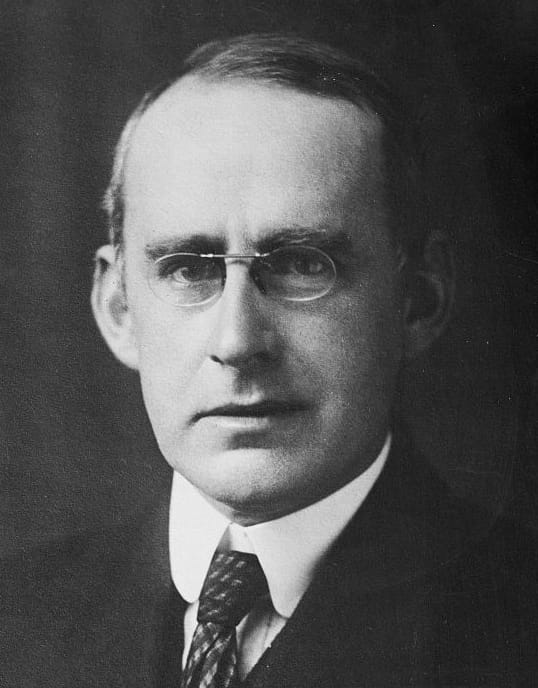
\includegraphics[width=.8\textwidth]{Images/Arthur_Stanley_Eddington.jpg}
            \end{figure}
            \begin{center}
                \Tiny{source : https://fr.wikipedia.org/wiki/Arthur\_Eddington}
            \end{center}
        \end{column}
        \begin{column}{.5\textwidth}
            "Nous rêvons parfois que l'homme saura un jour comment la libérer et l'utiliser pour ses propres besoins."\medskip\\
            $\qquad$- Arthur Eddington
        \end{column}
    \end{columns}
\end{frame}

\subsection{Motivation}

\begin{frame}{Introduction : Motivation}
    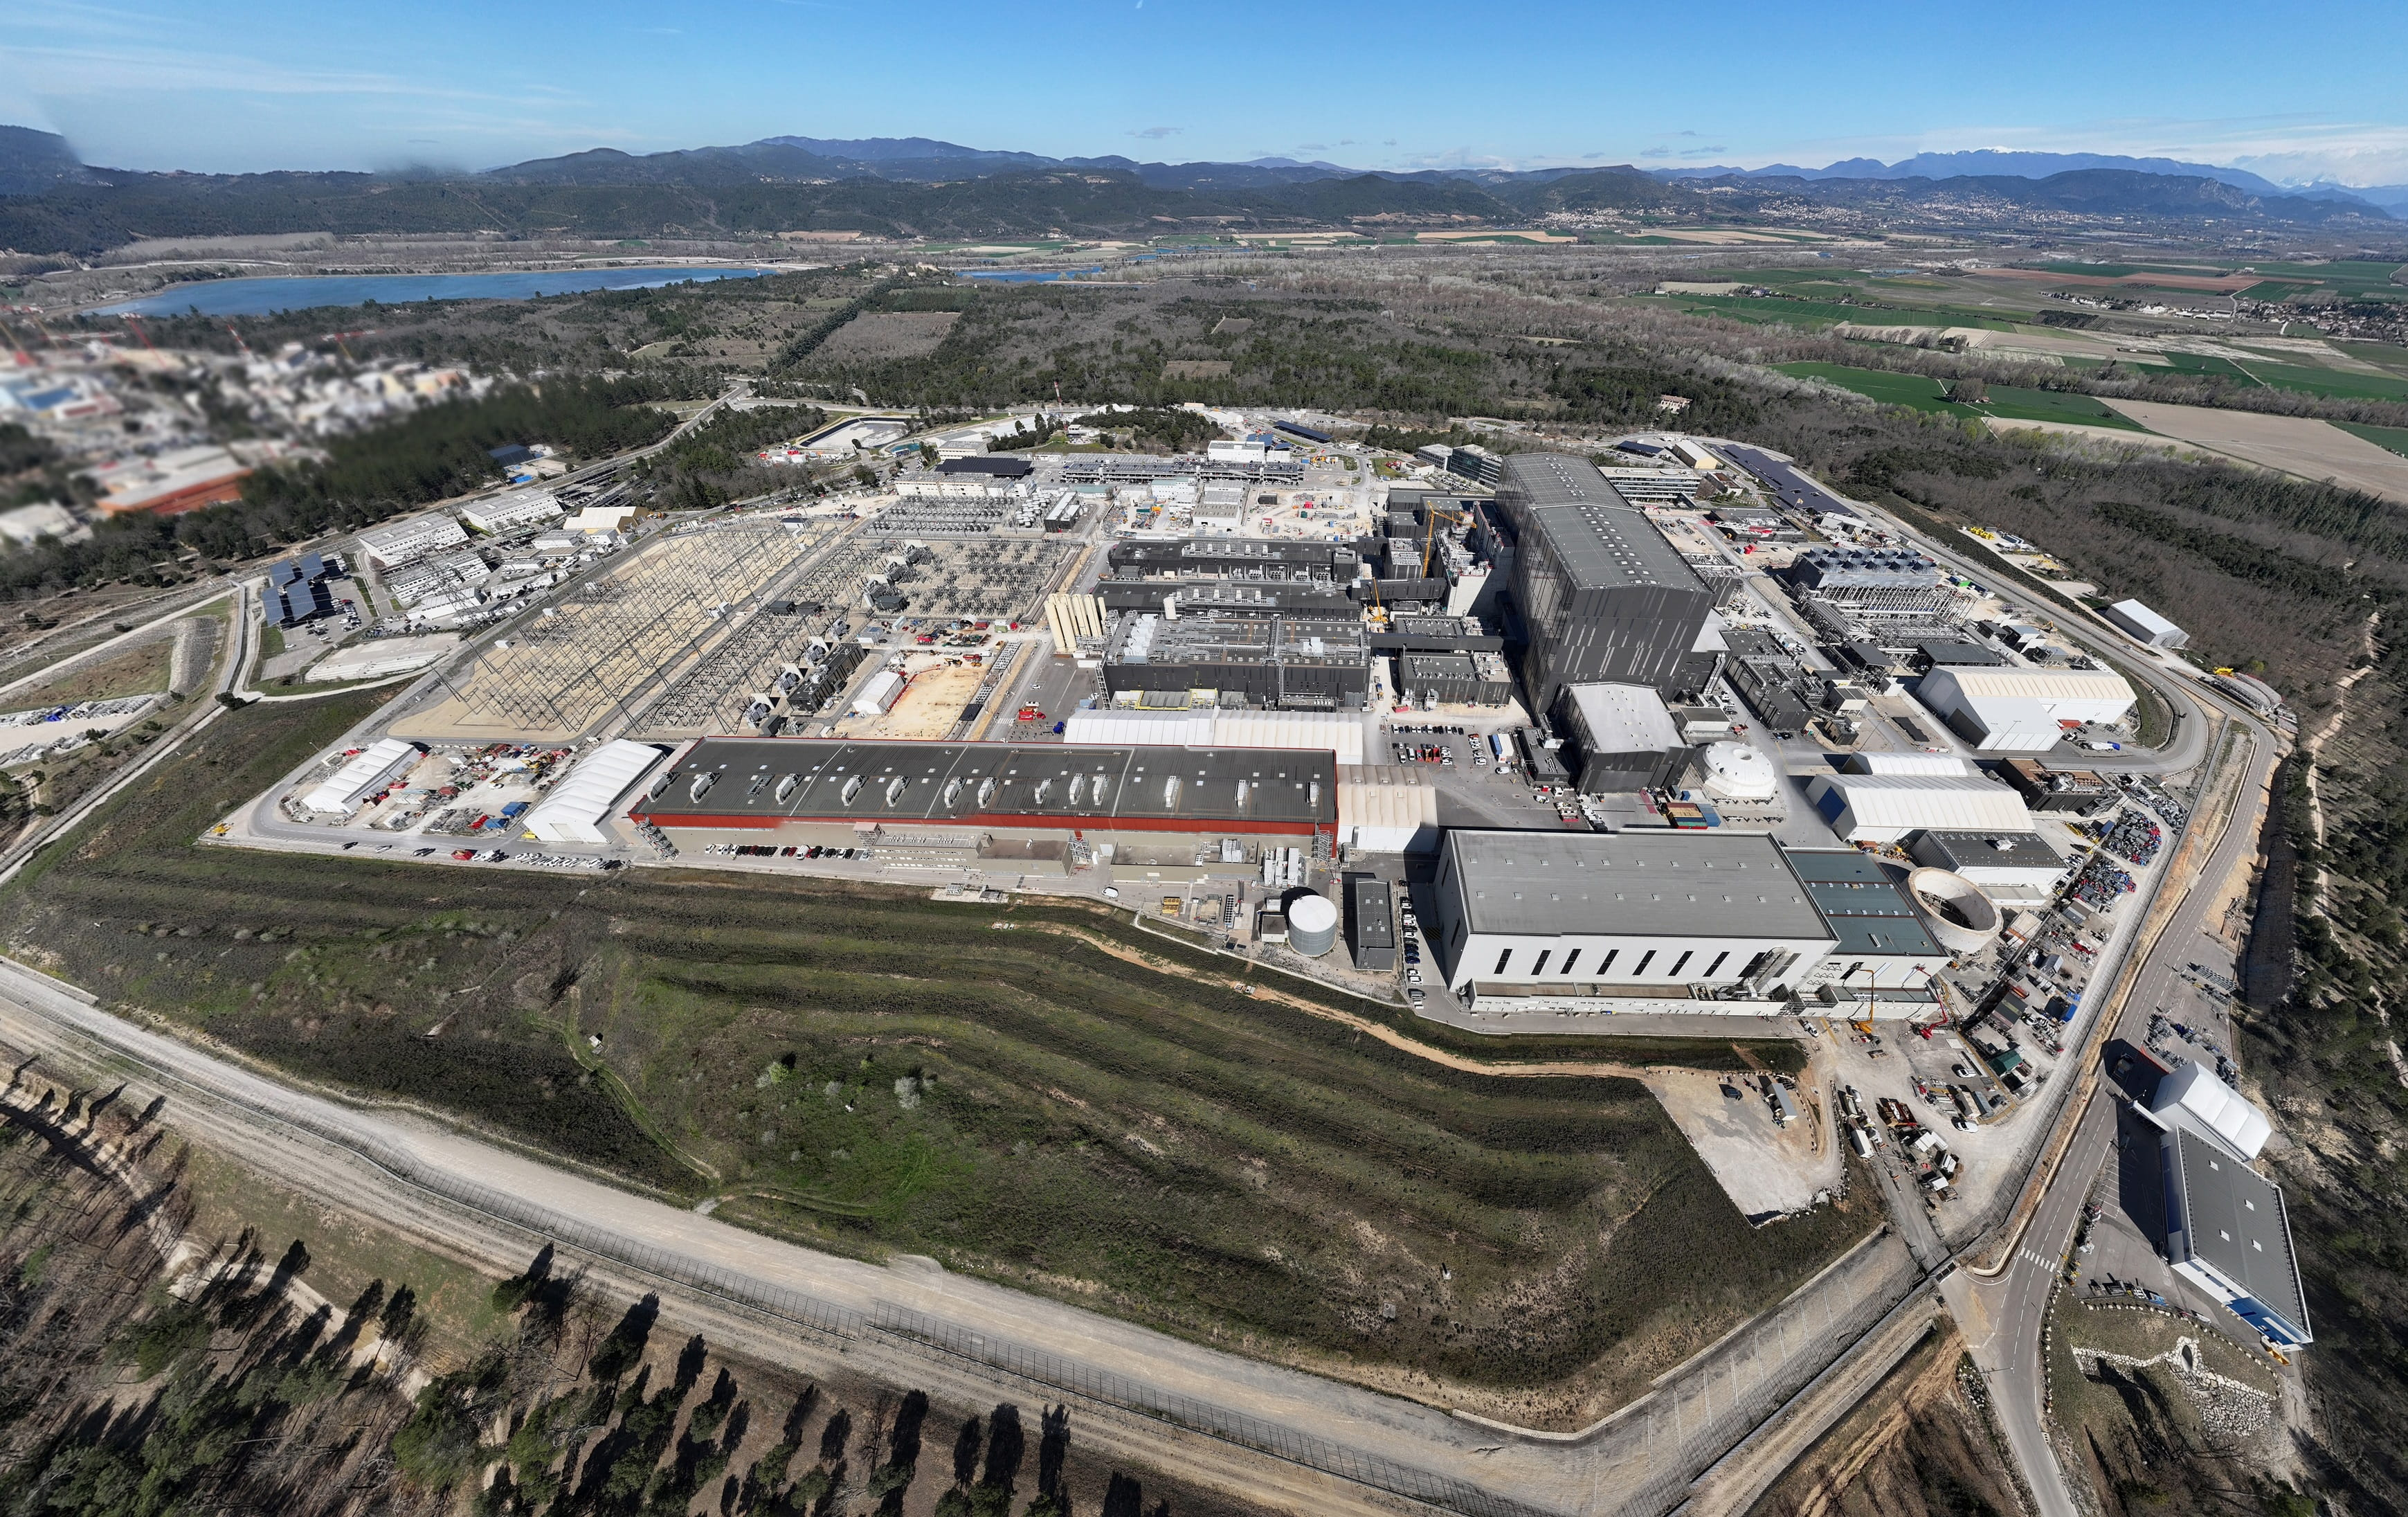
\includegraphics[width=.9\textwidth]{Images/dji_20260330111219_0135_d_panorama_sm.jpg}
\end{frame}

\subsection{Présentation d'ITER}

\begin{frame}{Introduction : Présentation d'ITER}
    \begin{columns}
        \begin{column}{.5\textwidth}
            \begin{figure}
                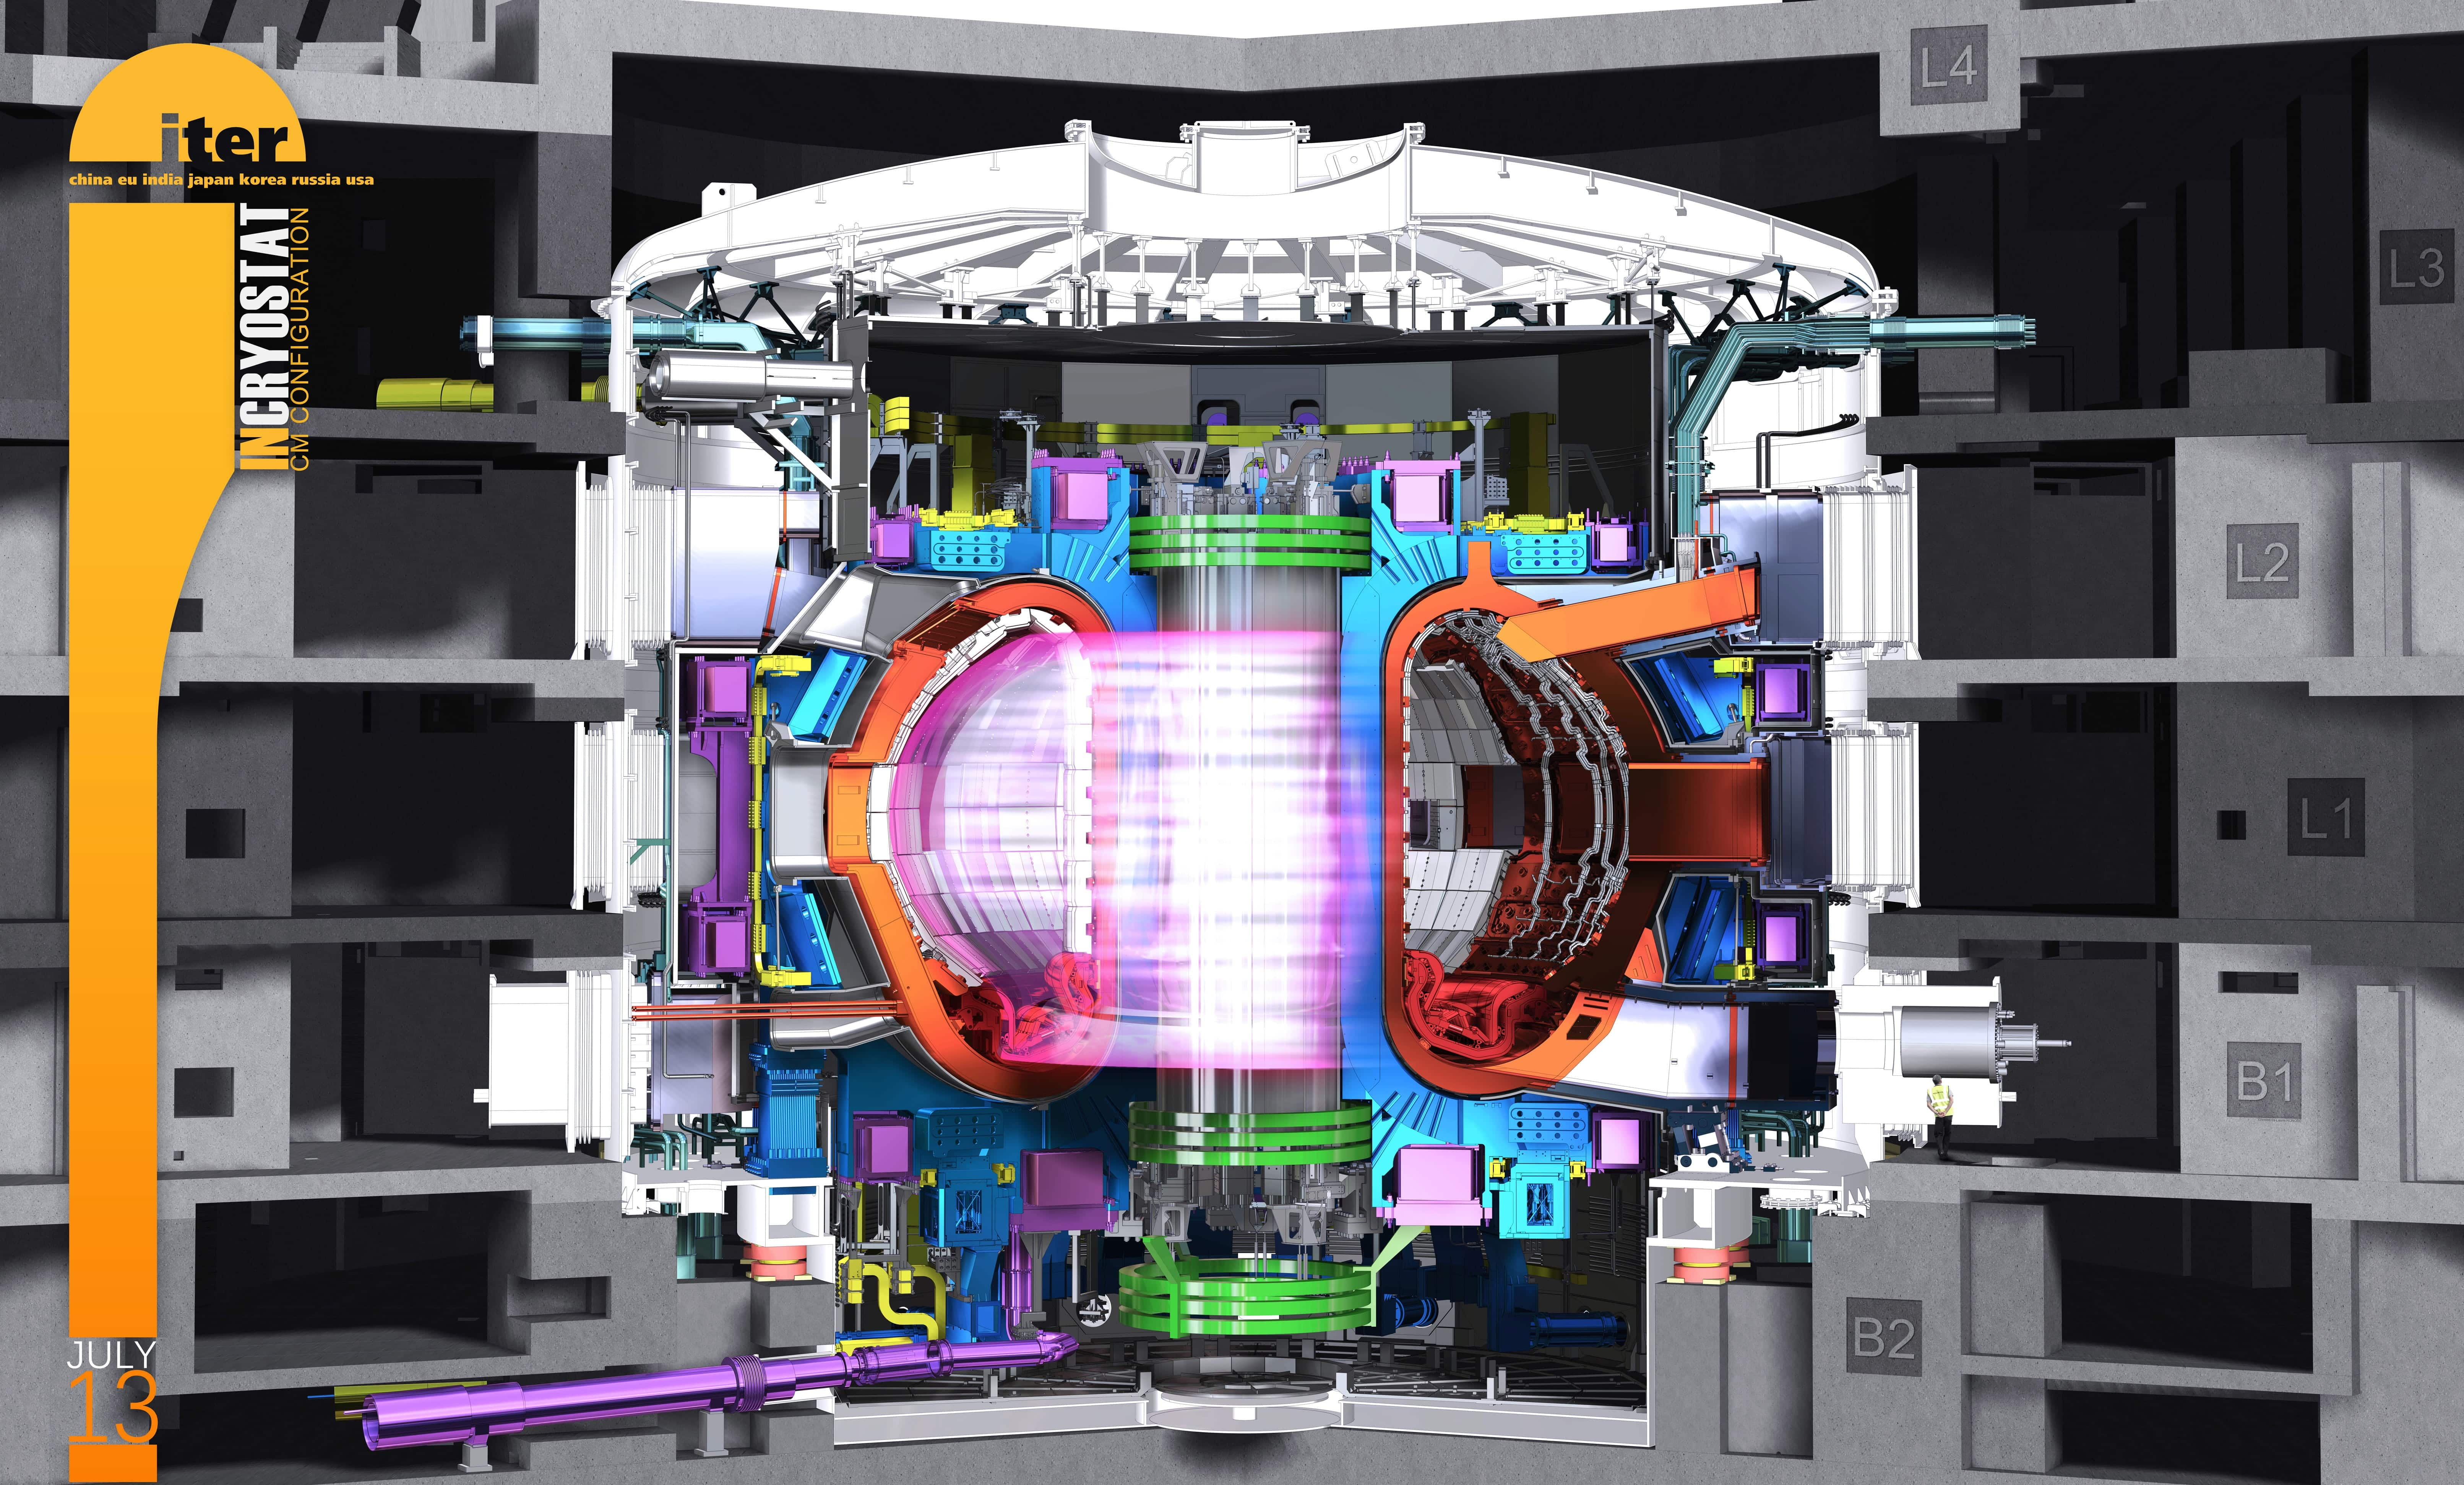
\includegraphics[width=1.1\linewidth]{Images/tkm_cplx_final_plasma2013-07.jpg}
            \end{figure}
            \begin{center}
                \Tiny{source : https://www.iter.org/few-lines}
            \end{center}
        \end{column}
        \begin{column}{.5\textwidth}
            \begin{itemize}
                \item \underline{Volume du plasma :} 840 m$^3$
                \item \underline{Température du plasma :} 150 millions de degré
                \item \underline{Puissance de chauffage :} 50 MW
                \item \underline{Attente de puissance} \underline{thermique :} 500 MW
            \end{itemize}
        \end{column}
    \end{columns}
\end{frame}

\subsection{Problématique}

\begin{frame}{Introduction : Problématique}
    \begin{center}
        \Large{Quelles sont les conditions nécessaires au maintien continu d'une réaction de fusion nucléaire dans un environnement confiné ?}
    \end{center}
\end{frame}

\subsection{Plan}

\begin{frame}{Introduction : Plan}
    \tableofcontents
\end{frame}

\section{Construction du modèle}

\subsection{Présentation de la simulation}

\begin{frame}{Construction du modèle}
    \begin{columns}
        \begin{column}{.5\textwidth}
            Réaction étudiée :
            \[ {}_1^2\text{D} + {}_1^3\text{T} \longrightarrow {}_2^4\text{He} + {}_0^1\text{n} + 17.59\text{ MeV} \]
        \end{column}
        \begin{column}{.5\textwidth}
            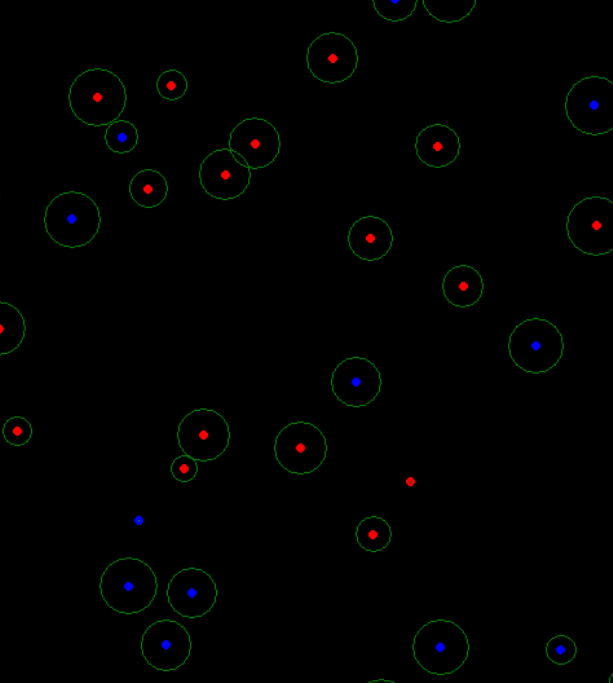
\includegraphics[width=1\textwidth]{Images/Image Code.png}
        \end{column}
    \end{columns}
    \begin{center}
        \tiny{Ligne 214 à 218 du script "Modélisation"}
    \end{center}
\end{frame}

\begin{frame}{"Cycle et boucle"}
    \begin{columns}
        \begin{column}{.5\textwidth}
            \begin{figure}
                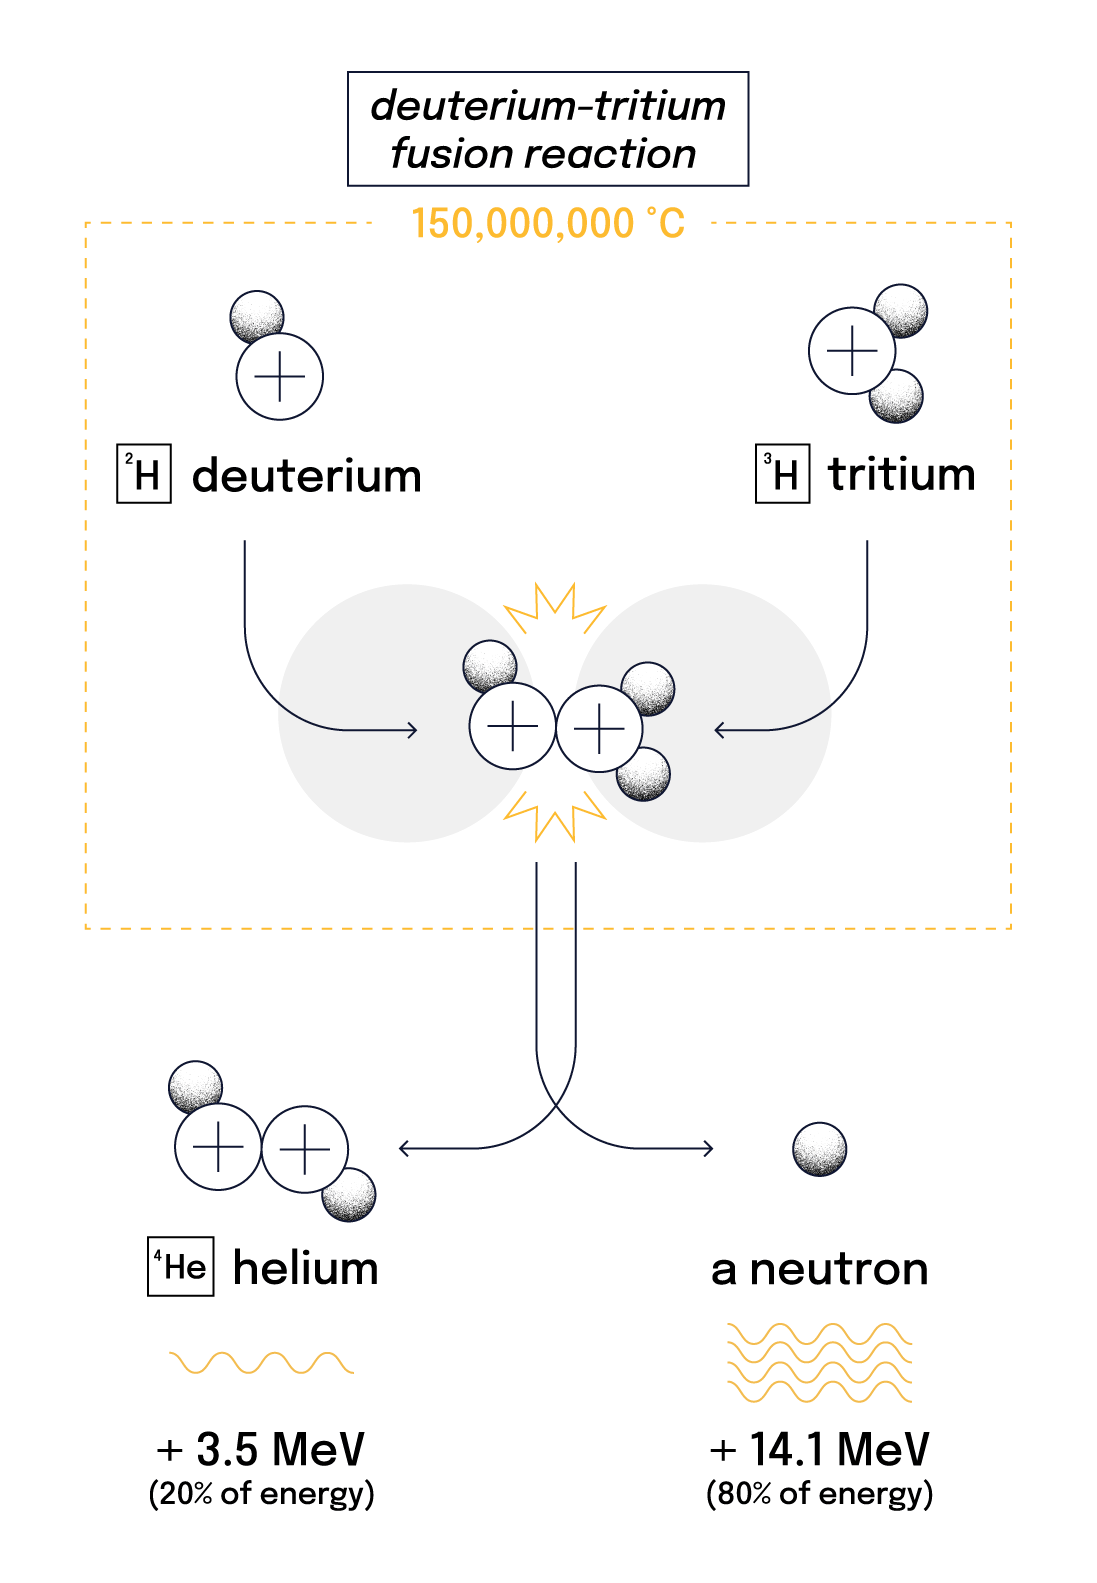
\includegraphics[width=.7\linewidth]{Images/deuterium-tritium-fusion-reaction_option1_2x_0.png}
            \end{figure}
            \begin{center}
                \Tiny{source : https://www.iter.org/fusion-energy/what-fusion}
            \end{center}
        \end{column}
        \begin{column}{.5\textwidth}
            Production du tritium dans le réacteur :
            \begin{figure}
                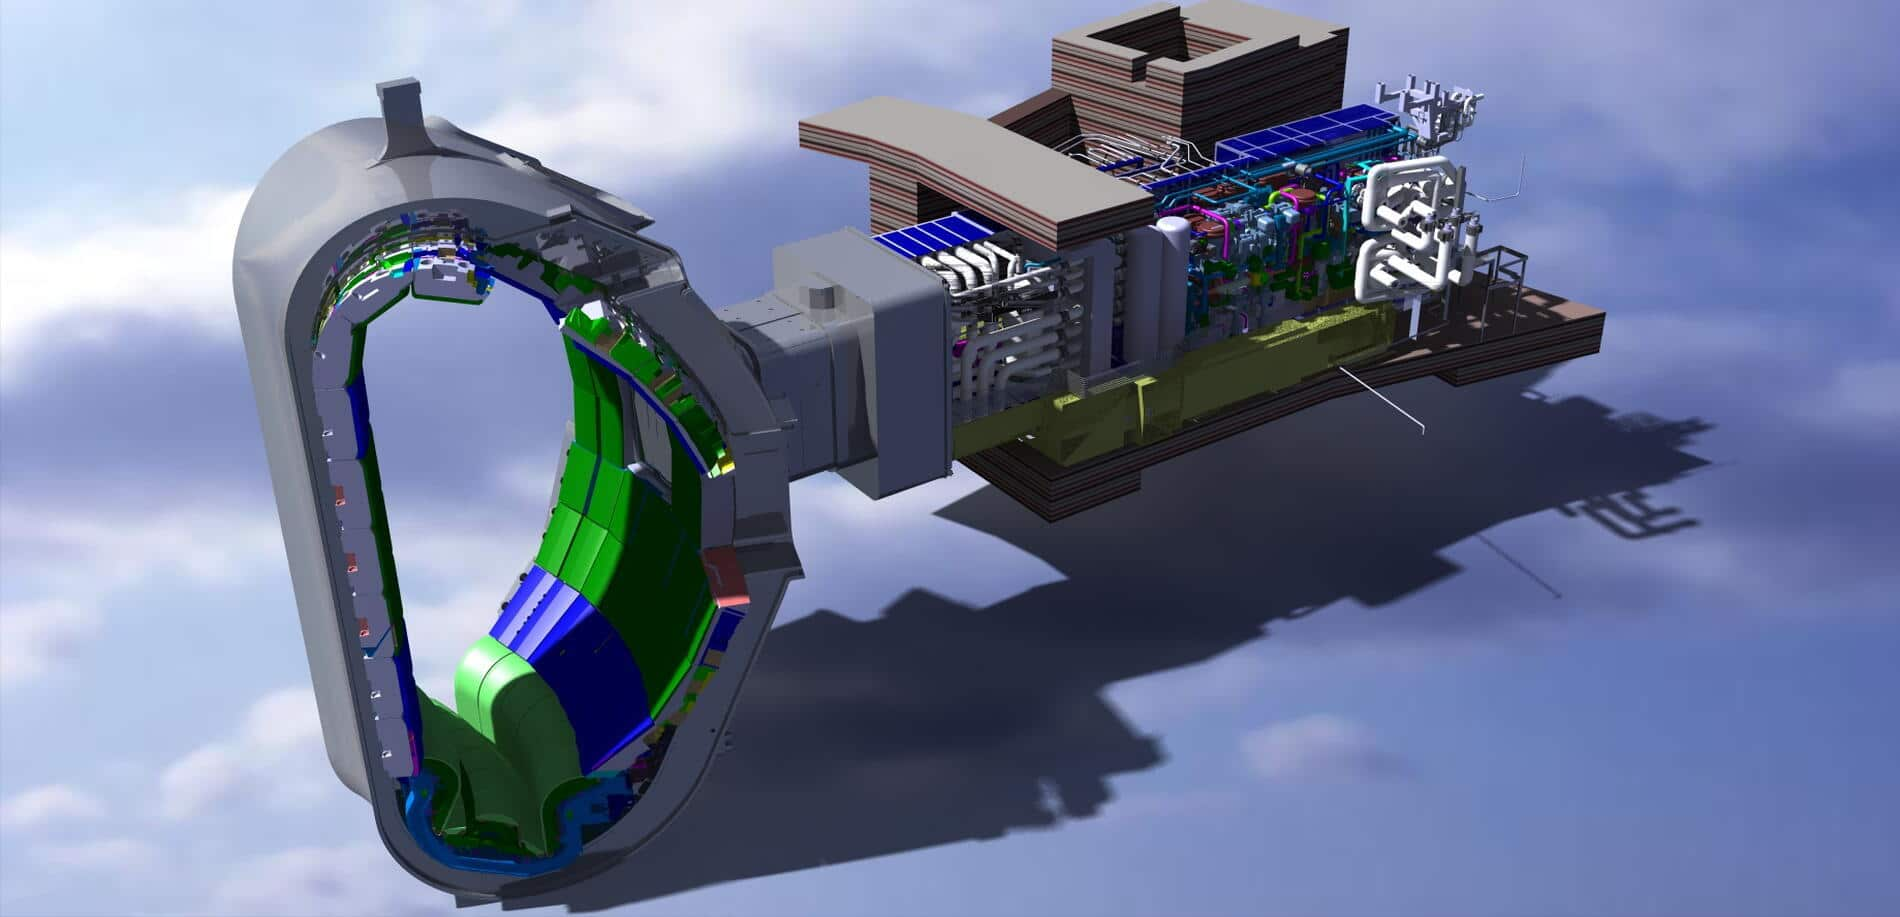
\includegraphics[width=1\linewidth]{Images/pic1-tbm_and_auxiliaries.jpg.jpg}
            \end{figure}
            \begin{center}
                \Tiny{source : https://www.iter.org/fr/machine/systemes-annexes/production-tritium}
            \end{center}
            \[ {}^6_3\text{Li} + {}_0^1\text{n} \longrightarrow {}_2^4\text{He} + {}_1^3\text{T} \]
        \end{column}
    \end{columns}
\end{frame}

\subsection{Force électrostatique}

\begin{frame}{Force électrostatique}
    \begin{columns}
        \begin{column}{.5\textwidth}
            Force électrostatique entre les particules :
            \[ \vec{F}_e = \frac{q^2}{4\pi\varepsilon_0}\times\frac{1}{r^2}\vec{u}_r \]
        \end{column}
        \begin{column}{.5\textwidth}
            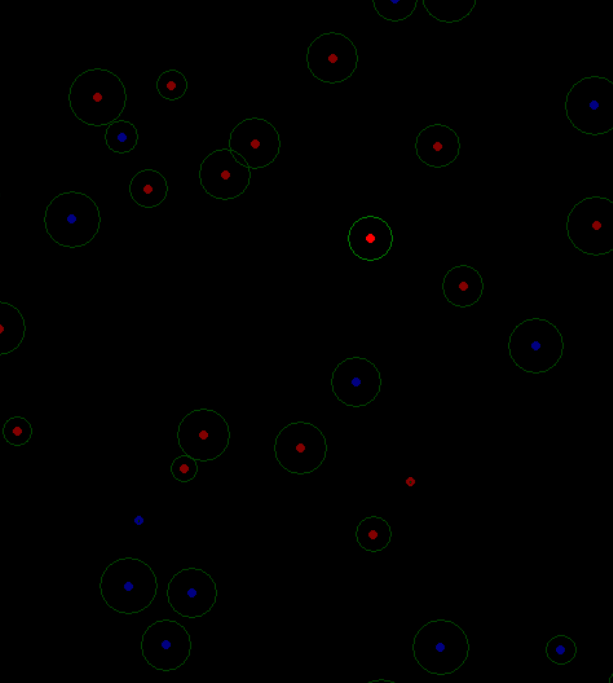
\includegraphics[width=1\textwidth]{Images/Image Code FE.png}
        \end{column}
    \end{columns}
    \begin{center}
        \tiny{Ligne 133 à 156 du script "Modélisation".}
    \end{center}
\end{frame}

\subsection{Section efficace}

\begin{frame}[fragile, allowframebreaks]{Section efficace}
    \begin{columns}
        \begin{column}{.5\textwidth}
            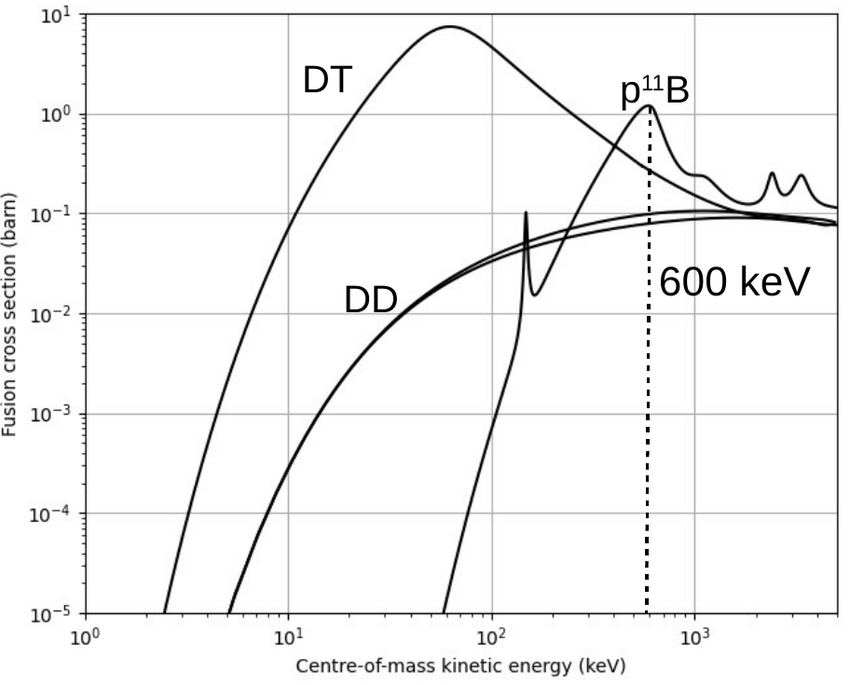
\includegraphics[width=1\textwidth]{Images/Fusion-cross-sections-of-Deuterium-Tritium-DT-Deuterium-Deuterium-DD-and.png}
            \begin{center}
                \Tiny{Multiscale study of high energy attosecond pulse interaction with matter and application to proton-Boron fusion (ResearchGate)}
            \end{center}
        \end{column}
        \begin{column}{.5\textwidth}
            Quantification de l'impact de l'effet tunnel sur la probabilité de fusion.
        \end{column}
    \end{columns}
    \framebreak
    \begin{columns}
        \begin{column}{.5\textwidth}
            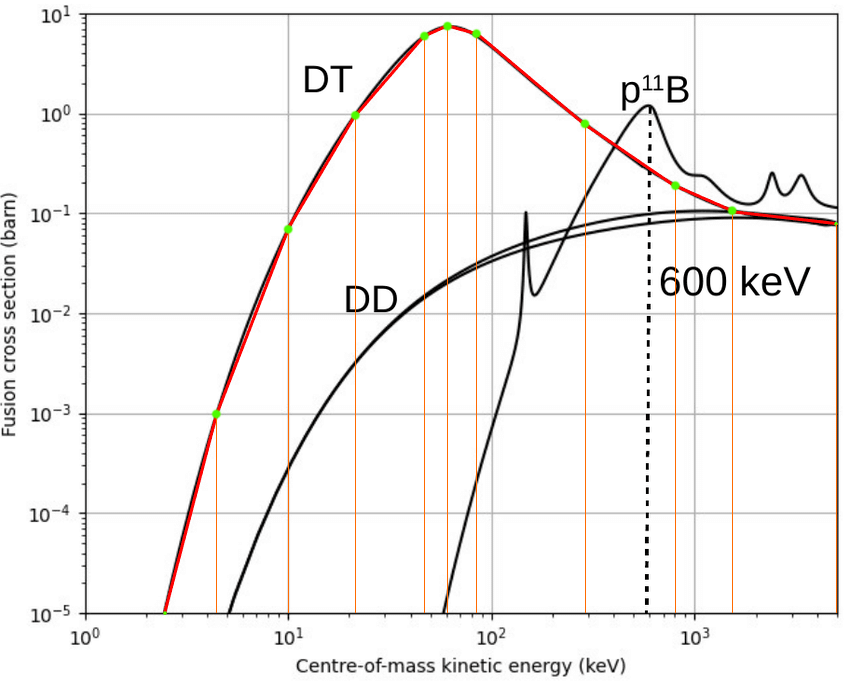
\includegraphics[width=1\textwidth]{Images/Fusion-cross-sections-of-Deuterium-Tritium-DT-Deuterium-Deuterium-DD-and(mod).png}
        \end{column}
        \begin{column}{.5\textwidth}
            Approximation par morceaux :
            \[ \ln(y) = \alpha\ln(x) + \beta \]
        \end{column}
    \end{columns}
    \begin{center}
        \tiny{Ligne 64 à 89 et 211 à 222 du script "Modélisation".}
    \end{center}
\end{frame}

\subsection{Distribution Maxwellienne des vitesses}

\begin{frame}{Construction du modèle}
    \begin{columns}
        \begin{column}{.5\textwidth}
            Distribution Maxwellienne des vitesses :
            \[ f(v) = \sqrt{\frac{2}{\pi}}\left(\frac{m}{k_BT}\right)^{\frac{3}{2}}v^2\mathrm{e}^{-\frac{mv^2}{2k_BT}} \]
        \end{column}
        \begin{column}{.5\textwidth}
            \begin{figure}
                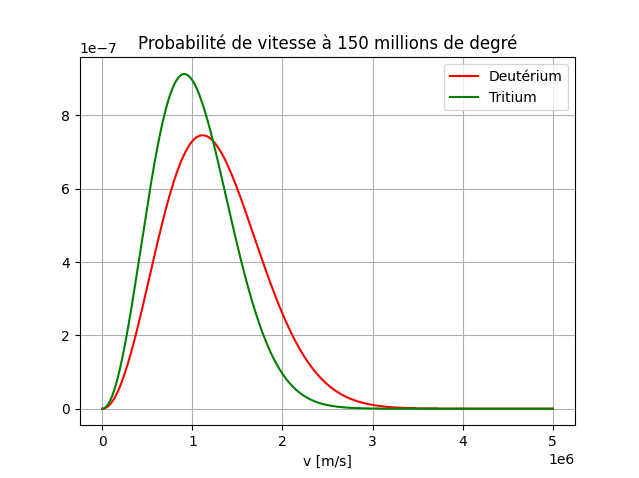
\includegraphics[width=1\linewidth]{Images/Probabilité de vitesse.png}
                \centering
            \end{figure}
        \end{column}
    \end{columns}
    \begin{center}
        \tiny{Ligne 42, 43 et 91 à 108 du script "Modélisation".}
    \end{center}
\end{frame}

\subsection{Énergie libérée}

\begin{frame}{Construction du modèle}
    On observe que lors de la réaction, on a :
    \begin{align*}
        \Delta m &= \underbrace{4.992722 m_p}_{m_d + m_t} - \underbrace{4.973974 m_p}_{m_{\text{He}} + m_n} \\
        &= 0.018747 m_p \\
        &\boxed{= 3.135790\times10^{-29}\text{ kg}}
    \end{align*}
    Ainsi, d'après la relation d'Einstein, on a :
    \begin{align*}
        E &= \Delta mc^2 \\
        &= 3.135790\times10^{-29}\times(2.9979\times10^8)^2 \\
        &\boxed{= 17.59\text{ MeV}}
    \end{align*}
    \begin{center}
        \tiny{Ligne 31 du script "Traitement des données".}
    \end{center}
\end{frame}

\section{La simulation}

\subsection{Les hypothèses}

\begin{frame}{La simulation}
    Hypothèses prises lors des simulations :
    \begin{itemize}
        \item Hélium éliminé instantanément
        \item Projection en 2 dimensions des particules
        \item Poids négligé
        \item 100 \% de l'énergie des neutrons est convertie en énergie thermique dans le plasma
        \item Température de 150 millions de degrés
        \item Tous les neutrons atteignent la couverture
        \item Critère de dégénérescence atteint
    \end{itemize}
\end{frame}

\subsection{Le fonctionnement}

\begin{frame}{Le fonctionnement I}
    \begin{figure}
        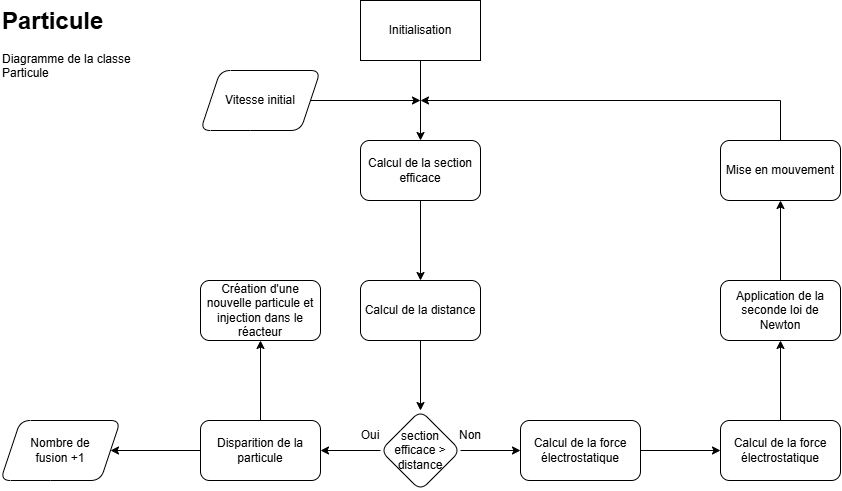
\includegraphics[scale=.35]{Images/Particules.drawio.png}
    \end{figure}
\end{frame}

\begin{frame}{Le fonctionnement II}
    \begin{figure}
        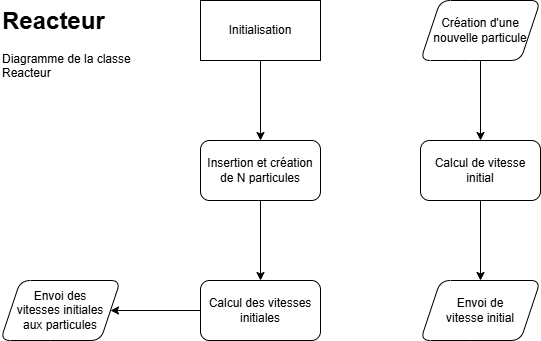
\includegraphics[width=.9\textwidth]{Images/Reacteur.drawio.png}
    \end{figure}
\end{frame}

\subsection{Résultats}

\begin{frame}[fragile, allowframebreaks]{Résultats}
    \begin{figure}
        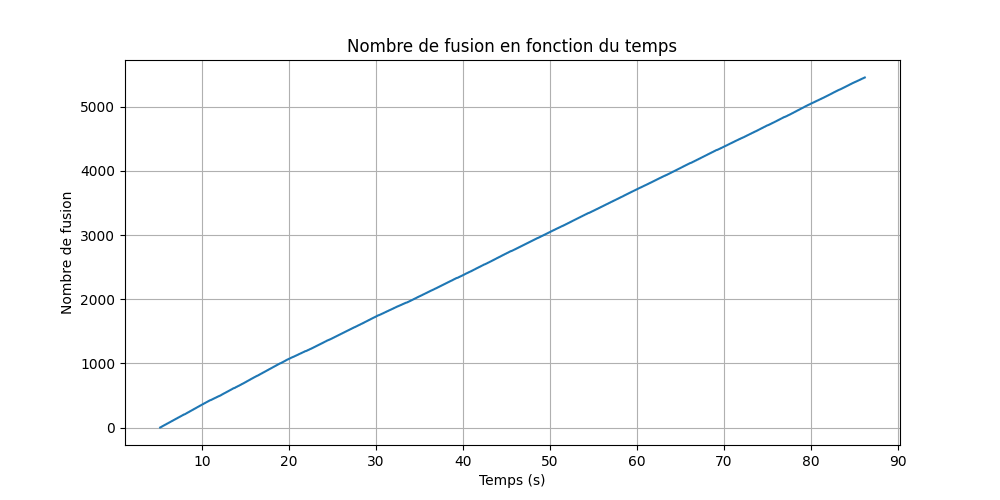
\includegraphics[width=1\textwidth]{Images/Avant traitement.png}
    \end{figure}
    \framebreak
    \begin{figure}
        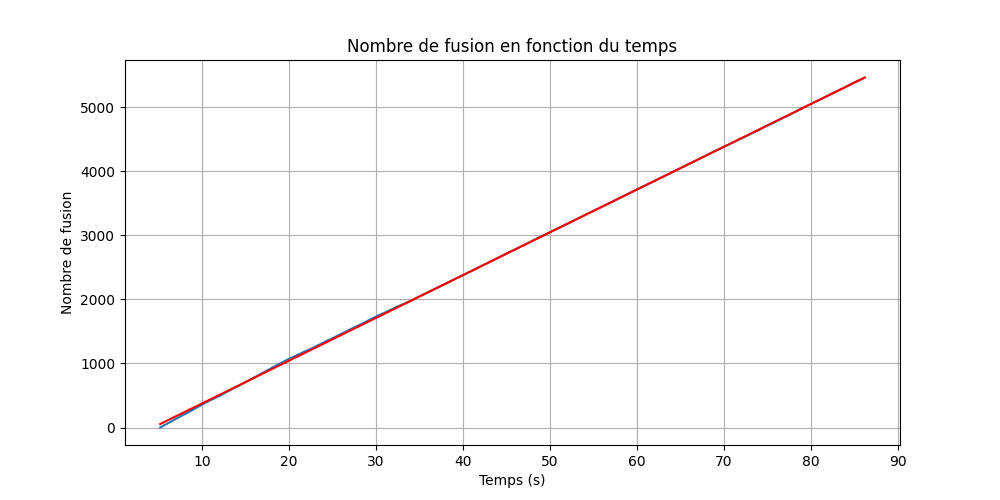
\includegraphics[width=1\textwidth]{Images/Apres traitement.png}
    \end{figure}
    \[ y = ax + b \]

    \framebreak
    Obtention de la puissance :
    \[ P = a\times14.1\text{ MeV}\times\frac{840\text{ m}^3}{V} \]
    On obtient donc :
    \[ \boxed{P = 632\text{ MW}} \]
\end{frame}

\section{Comparaison avec ITER}

\begin{frame}{Comparaison avec ITER I}
    Différences entre les simulations :
    \begin{columns}
        \begin{column}{.49\textwidth}
            \begin{center}
                TIPE :
            \end{center}
            \begin{itemize}
                \item 2D
                \item Hélium éliminé instantanément
                \item Non prise en compte du rayonnement
                \item Non prise en compte du temps de confinement
            \end{itemize}
            \[ P = 632\text{ MW} \]
        \end{column}
        \begin{column}{.02\textwidth}
            \rule{.1mm}{0.7\textheight}
        \end{column}
        \begin{column}{.49\textwidth}
            \begin{center}
                Fusion for Energy (F4E) :
            \end{center}
            \begin{itemize}
                \item 3D
                \item Modélisation du divertor
                \item Prise en compte du rayonnement
                \item Prise en compte du temps de confinement
            \end{itemize}
            \[ P = 500\text{ MW} \]
        \end{column}
    \end{columns}
\end{frame}

\begin{frame}{Comparaison avec ITER II}
    Avec des hypothèse similaires
    \begin{columns}
        \begin{column}{.49\textwidth}
            \begin{center}
                TIPE :
            \end{center}
            \begin{itemize}
                \item 2D
                \item Hélium éliminé instantanément
                \item Non prise en compte du rayonnement
                \item Non prise en compte du temps de confinement
            \end{itemize}
            \[ P = 632\text{ MW} \]
        \end{column}
        \begin{column}{.02\textwidth}
            \rule{.1mm}{0.65\textheight}
        \end{column}
        \begin{column}{.49\textwidth}
            \begin{center}
                Fusion For Energy (F4E) :
            \end{center}
            \begin{itemize}
                \item 3D
                \item Hélium éliminé instantanément
                \item Non prise en compte du rayonnement
                \item Non prise en compte du temps de confinement
            \end{itemize}
            \[ P = 640\text{ MW} \]
        \end{column}
    \end{columns}
\end{frame}

\section{Conclusion}

\begin{frame}{Conclusion}
    Quelles sont les conditions nécessaires au maintien continu d’une réaction de fusion nucléaire dans un environnement confiné ?\medskip
    \begin{itemize}
        \item 150 millions de degrés
        \item 840 m$^3$
        \item Densité de l'ordre de $10^{22}$
    \end{itemize}
\end{frame}

\begin{frame}
    "La fusion nucléaire n'est peut-être pas l'énergie du futur, mais c'est une voie qui mérite d'être explorée."
    \begin{flushright}
        Un ingénieur chez F4E
    \end{flushright}\bigskip\bigskip\bigskip

    \begin{center}
        \Large{\textbf{***}}
    \end{center}
\end{frame}

\section[]{Annexe}

\subsection{Distribution Maxwellienne des vitesses}

\begin{frame}[fragile, allowframebreaks, t]{Annexe : Distribution Maxwelienne des vitesses}
    On cherche à cacluler l'intégrale suivante :
    \[ I = \int_0^{+\infty}\sqrt{\frac{2}{\pi}}\left(\frac{m}{k_BT}\right)^\frac{3}{2}v^2\mathrm{e}^{-\frac{mv^2}{2k_BT}}\dint{v} \]
    Pour cela, on pose $\displaystyle a=\sqrt{\frac{2}{\pi}}\left(\frac{m}{k_BT}\right)^\frac{3}{2}$ et $\displaystyle b=\frac{m}{2k_BT}$. On obtient donc :
    \[ I = a\int_0^{+\infty}v^2\e^{-bv^2}\dint{v} \]
    On pose pour $\n^*,\ f_n:\begin{array}[t]{rcl}
        \R&\to&\R\\x&\mapsto&\left(1+\frac{bx^2}{n}\right)^{-n}
    \end{array}$ continue par morceaux sur $\R$. \\
    La suite $(f_n)$ converge simplement vers $f:x\mapsto\e^{-bx^2}$ continue par morceaux sur $\R$. \\
    D'après la formule du binôme de Newton, pour tout $\n^*$ et pour tout $x\in\R_+$, on a :
    \begin{align*}
        \left(1+\frac{bx^2}{n}\right)^n &= \sum_{k=0}^n\binom{n}{k}\frac{b^kx^{2k}}{n^k} \\
        &\geqslant 1 + n\times\frac{bx^2}{n} \\
        &= 1 + bx^2
    \end{align*}
    Donc $\displaystyle|f_n(x)|\leqslant\frac{1}{1+bx^2}$ et $\displaystyle x\mapsto\frac{1}{1+bx^2}\in L^1(\R_+)$. \\
    Donc d'après le théorème de convergence dominée :
    \[ \int_0^{+\infty}f_n\dint{x}\quad\toinf{n}\quad\int_0^{+\infty}\e^{-bx^2}\dint{x} \]
    Il reste à calculer l'intégrale de $f_n$ pour $\n^*$. \\
    Soit $\n^*$. \\
    On effectue le changement de variable $\displaystyle t=\frac{x\sqrt{b}}{\sqrt{n}}\ \left(\dint{t}=\frac{\sqrt{b}}{\sqrt{n}}\dint{x}\right)$
    \begin{align*}
        \int_0^{+\infty}f_n(x)\dint{x} &= \int_0^{+\infty}(1+t^2)^{-n}\frac{\sqrt{n}}{\sqrt{b}}\dint{t} \\
        &= \sqrt{\frac{n}{b}}\int_0^{+\infty}\frac{1}{(1+t^2)^n}\dint{t}
    \end{align*}
    On effectue le changement de variable $\displaystyle u=\arctan(t)\ \left(\dint{u}=\frac{1}{1+t^2}\dint{t}\right)$. Donc
    \begin{align*}
        \sqrt{\frac{n}{b}}\int_0^{+\infty}\frac{1}{(1+t^2)^n}\dint{t} &= \sqrt{\frac{n}{b}}\int_0^{\frac{\pi}{2}}\frac{1}{(1+\tan^2(u))^{n-1}}\dint{u} \\
        &= \sqrt{\frac{n}{b}}\int_0^{\frac{\pi}{2}}\cos^{2(n-1)}\dint{u} \\
        &= \sqrt{\frac{n}{b}}W_{2(n-1)}
    \end{align*}
    On reconnait les intégrales de Wallis. \\
    On a donc $W_{n}\simp\sqrt{\frac{\pi}{2n}}$. \\
    Donc
    \begin{align*}
        \sqrt{\frac{n}{b}}W_{2(n-1)}&\simp\sqrt{\frac{n}{b}}\sqrt{\frac{\pi}{4n-4}} \\
        &\simp \frac{\sqrt{\pi}}{2\sqrt{b}}
    \end{align*}
    Finalement,
    \[ \int_0^{+\infty}f_n(x)\dint{x}\simp\frac{\sqrt{\pi}}{2\sqrt{b}} \]
    Donc :
    \[ \int_0^{+\infty}\e^{-bx^2}\dint{x} = \frac{\sqrt{\pi}}{2\sqrt{b}} \]
    D'où :
    \[ \int_0^{+\infty}a\e^{-bx^2}\dint{x} = \frac{a\sqrt{\pi}}{2\sqrt{b}} \tag{1} \]
    On pose, pour $x\in\R_+$ et $b\in\R,\ g:(x,b)\mapsto a\e^{-bx^2}$. \\
    Pour tout $x\in\R_+,\ g:b\mapsto\e^{-bx^2}$ est continue et dérivable sur $\R$. \\
    Pour tout $b\in\R,\ g:x\mapsto\e^{-bx^2}$ est continue par morceaux sur $\R_+$ \\
    Pour tout $x\in\R_+,\ \displaystyle\frac{\partial f}{\partial b}(x, b) = -ax^2\e^{-bx^2}$ continue par morceaux sur $\R$. \\
    Donc, d'après (1) :
    \[ I = \int_0^{+\infty}ax^2\e^{-bx^2} = \frac{a\sqrt{\pi}}{4b\sqrt{b}} \]
    Or $\displaystyle a=\sqrt{\frac{2}{\pi}}\left(\frac{m}{k_BT}\right)^\frac{3}{2}$ et $\displaystyle b=\frac{m}{2k_BT}$. Donc
    \begin{align*}
        \frac{a}{b\sqrt{b}} &= \frac{\sqrt{\frac{2}{\pi}}\left(\frac{m}{k_BT}\right)^\frac{3}{2}}{\frac{m}{2k_BT}\sqrt{\frac{m}{2k_BT}}} \\
        &= \frac{\sqrt{\frac{2}{\pi}}m^{\frac{3}{2}}(2k_BT)^{\frac{3}{2}}}{(k_BT)^{\frac{3}{2}}m\sqrt{m}} \\
        &= \frac{4}{\sqrt{\pi}}
    \end{align*}
    D'où
    \[ \boxed{I = 1} \]
\end{frame}

\subsection{Critère de dégénérescence}

\begin{frame}[fragile, allowframebreaks]{Annexe : Critère de dégénérescence}
    La longueur d'onde thermique de de Broglie est définit par :
    \[ \boxed{\lambda_\text{th} = \frac{h}{\sqrt{2\pi mk_BT}}} \]
    Dans notre cas, on a :
    \begin{itemize}
        \item $T = 1.5\times10^8$ K \\
        \item $m_d = 3.34\times10^{-27}$ kg et $m_t = 5.00\times10^{-27}$ kg
    \end{itemize}
    Ainsi, on a :
    \begin{align*}
        \lambda_\text{th, d} &= \frac{6.62\times10^{-34}}{\sqrt{2\times3.14\times3.34\times10^{-27}\times1.38\times10^{-23}\times1.5\times10^8}} \\
        &= 1.005\times10^{-13}\text{ m}
    \end{align*}
    Et :
    \begin{align*}
        \lambda_\text{th, t} &= \frac{6.62\times10^{-34}}{\sqrt{2\times3.14\times5.00\times10^{-27}\times1.38\times10^{-23}\times1.5\times10^8}} \\
        &= 8.215\times10^{-14}\text{ m}
    \end{align*}
    De plus, la densité d'un système quantique est définit par :
    \[ \boxed{\rho = \frac{N}{V}} \]
    Avec $N$ le nombre de particule et $V$ le volume du système. \\
    Dans notre cas, on a :
    \begin{itemize}
        \item $N = 4.2\times10^{22}$
        \item $V = 840$ m$^3$
    \end{itemize}
    Ainsi, on a :
    \begin{align*}
        \rho &= \frac{4.2\times10^{22}}{840} \\
        &= 5\times10^{19}\text{ m}^{-3}
    \end{align*}
    D'après le critère de dégénérécence, si la limite classique est atteinte, on a :
    \[ \rho\lambda_\text{th}^3\ll1 \]
    Dans le pire des cas, on a :
    \begin{align*}
        \rho\lambda_\text{th, d}^3 &= 5\times10^{19}\times\Big(1.005\times10^{-13}\Big)^3 \\
        &= 5\times1.015\times10^{-20} \\
        &\sim10^{-20}
    \end{align*}
    On a donc :
    \[ \rho\lambda_\text{th}^3\sim10^{-20}\ll1 \]
\end{frame}

\subsection{Ordre de grandeur}

\begin{frame}{Annexe : Ordre de grandeur}
    \begin{itemize}
        \item Vitesse moyenne des particules dans le réacteur : $10^6\text{ m.s}^{-1}$.
        \item Vitesse d'éjection de l'électron : $10^7\text{ m.s}^{-1}$
        \item Vitesse d'éjection de l'hélium : $10^7\text{ m.s}^{-1}$
        \item Champ magnétique dans la chambre : $13$ T
        \item Courant parcourant les aimants : entre $10$ kA et $5$ MA.
    \end{itemize}
\end{frame}

\subsection{Critère de Lawson}

\begin{frame}{Annexe : Critère de Lawson}
    \begin{columns}
        \begin{column}{.5\textwidth}
            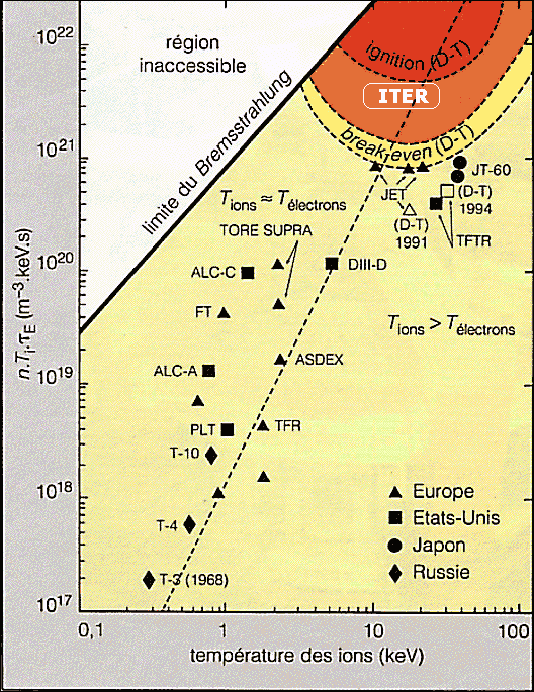
\includegraphics[width=.85\textwidth]{Images/lawson.png}
            \begin{center}
                \Tiny{source : https://www.nucleaire-info.com/critere\_de\_lawson.htm}
            \end{center}
        \end{column}
        \begin{column}{.5\textwidth}
            On note :
            \begin{itemize}
                \item $T$ : la température du plasma
                \item $\tau$ : le temps de confinement
                \item $n$ : la densité
            \end{itemize}
            Le critère de Lawson est :
            \[ n\tau T > 5\times10^{21}\text{ m}^{-3}.\text{keV.s} \]
        \end{column}
    \end{columns}
\end{frame}

\subsection{Code}

\subsubsection{Modélisation}

\begin{frame}[fragile, allowframebreaks]{Annexe : Code - Modélisation}
    \lstinputlisting{/home/thomas/Documents/Cours/TIPE/Code/V20.py}
\end{frame}

\subsubsection{Traitement des données}

\begin{frame}[fragile, allowframebreaks]{Annexe : Code - Traitement des données}
    \lstinputlisting{/home/thomas/Documents/Cours/TIPE/Code/Traitement des donnees.py}
\end{frame}

\subsubsection{Tracer de courbe}

\begin{frame}[fragile]{Annexe : Code - Tracer de courbe}
    \lstinputlisting{/home/thomas/Documents/Cours/TIPE/Code/graph.py}
\end{frame}

\end{document}